\subsection{The Significance of Incorrect assumptions on the (In-)Completeness of the Data Set} \label{sec:results_incompR}

The selection function of a survey could be described by a spatial survey volume and a completeness function, which determines the fraction of stars observed at a given location within the Galaxy with a given brightness, metallicity etc (see \S\ref{sec:selectionfunction}). The completeness function depends on the characteristics and mode of the survey, can be very complex and is therefore sometimes not perfectly known. We investigate how much an imperfect knowledge of the selection function can affect the recovery of the potential. We model this by creating mock data with varying incompleteness, while assuming constant completeness in the analysis. The mock data comes from a sphere around the sun and an incompleteness function that drops linearly with distance $r$ from the sun (see Test \ref{test:isoSphFlexIncomp}, Example 1, in Table \ref{tbl:tests} and Figure \ref{fig:isoSphFlexIncompR_mockdata}).
\\This could be understood as a model for the important effect of stars being less likely to be observed the further away they are. We demonstrate that the potential recovery with \RM is very robust against somewhat wrong assumptions about the (in-)completeness of the data (see Figure \ref{fig:isoSphFlexIncompR_violins}). A lot of information about the potential comes from the rotation curve measurements in the plane, which is not affected by applying an incompleteness function. In Appendix \S\ref{sec:incompZ} we also show that the robustness is somewhat less striking but still given for small misjudgments of the incompleteness in vertical direction, parallel to the disk plane (Figures \ref{fig:isoSphFlexIncompZ_mockdata} and \ref{fig:isoSphFlexIncompZ_violins}). This could model the effect of wrong corrections for dust obscuration in the plane. We also investigate in Appendix \S\ref{sec:incompZ} if indeed most of the information is stored in the rotation curve. For this we use the same mock data sets as analysed in Figures \ref{fig:isoSphFlexIncompR_violins} and \ref{fig:isoSphFlexIncompZ_violins}, but this time we’re not including the tangential velocities in the modelling, rather marginalizing the likelihood over $v_T$. In this case the potential is much less tightly constrained, even for 20,000 stars. For only small deviations of true and assumed completeness ($\lesssim 10\%$) we can however still incorporate the true potential in our fitting result (see Figure \ref{fig:isoSphFlexIncomp_marginal_violins}). 



%FIGURE: isoSphFlexIncompR in mock data space

\begin{figure}
\includegraphics[width=\columnwidth]{figs/isoSphFlexIncompR_mockdata.eps}
\caption{Selection function and mock data distribution for investigating radial incompleteness of the data. All model parameters are summarized as Test \ref{test:isoSphFlexIncomp}, Example 1, in Table \ref{tbl:tests}. The survey volume is a sphere around the sun and the percentage of observed stars is decreasing linearly with radius from the sun, as demonstrated in the left panel. How fast this detection/incompleteness rate drops is quantified by the factor $\epsilon_r$. Histograms for four data sets, drawn from two \MAPs{} (\texttt{hot} in red and \texttt{cool} in blue, see Table \ref{tbl:referenceMAPs}) and with two different $\epsilon_r$, 0 and 0.7, are shown in the right panel for illustration purposes. [TO DO: Potential and/or population names in typewriter font]} 
\label{fig:isoSphFlexIncompR_mockdata}
\end{figure}

%FIGURE: isoSphFlexIncompR

\begin{figure*}
\centering
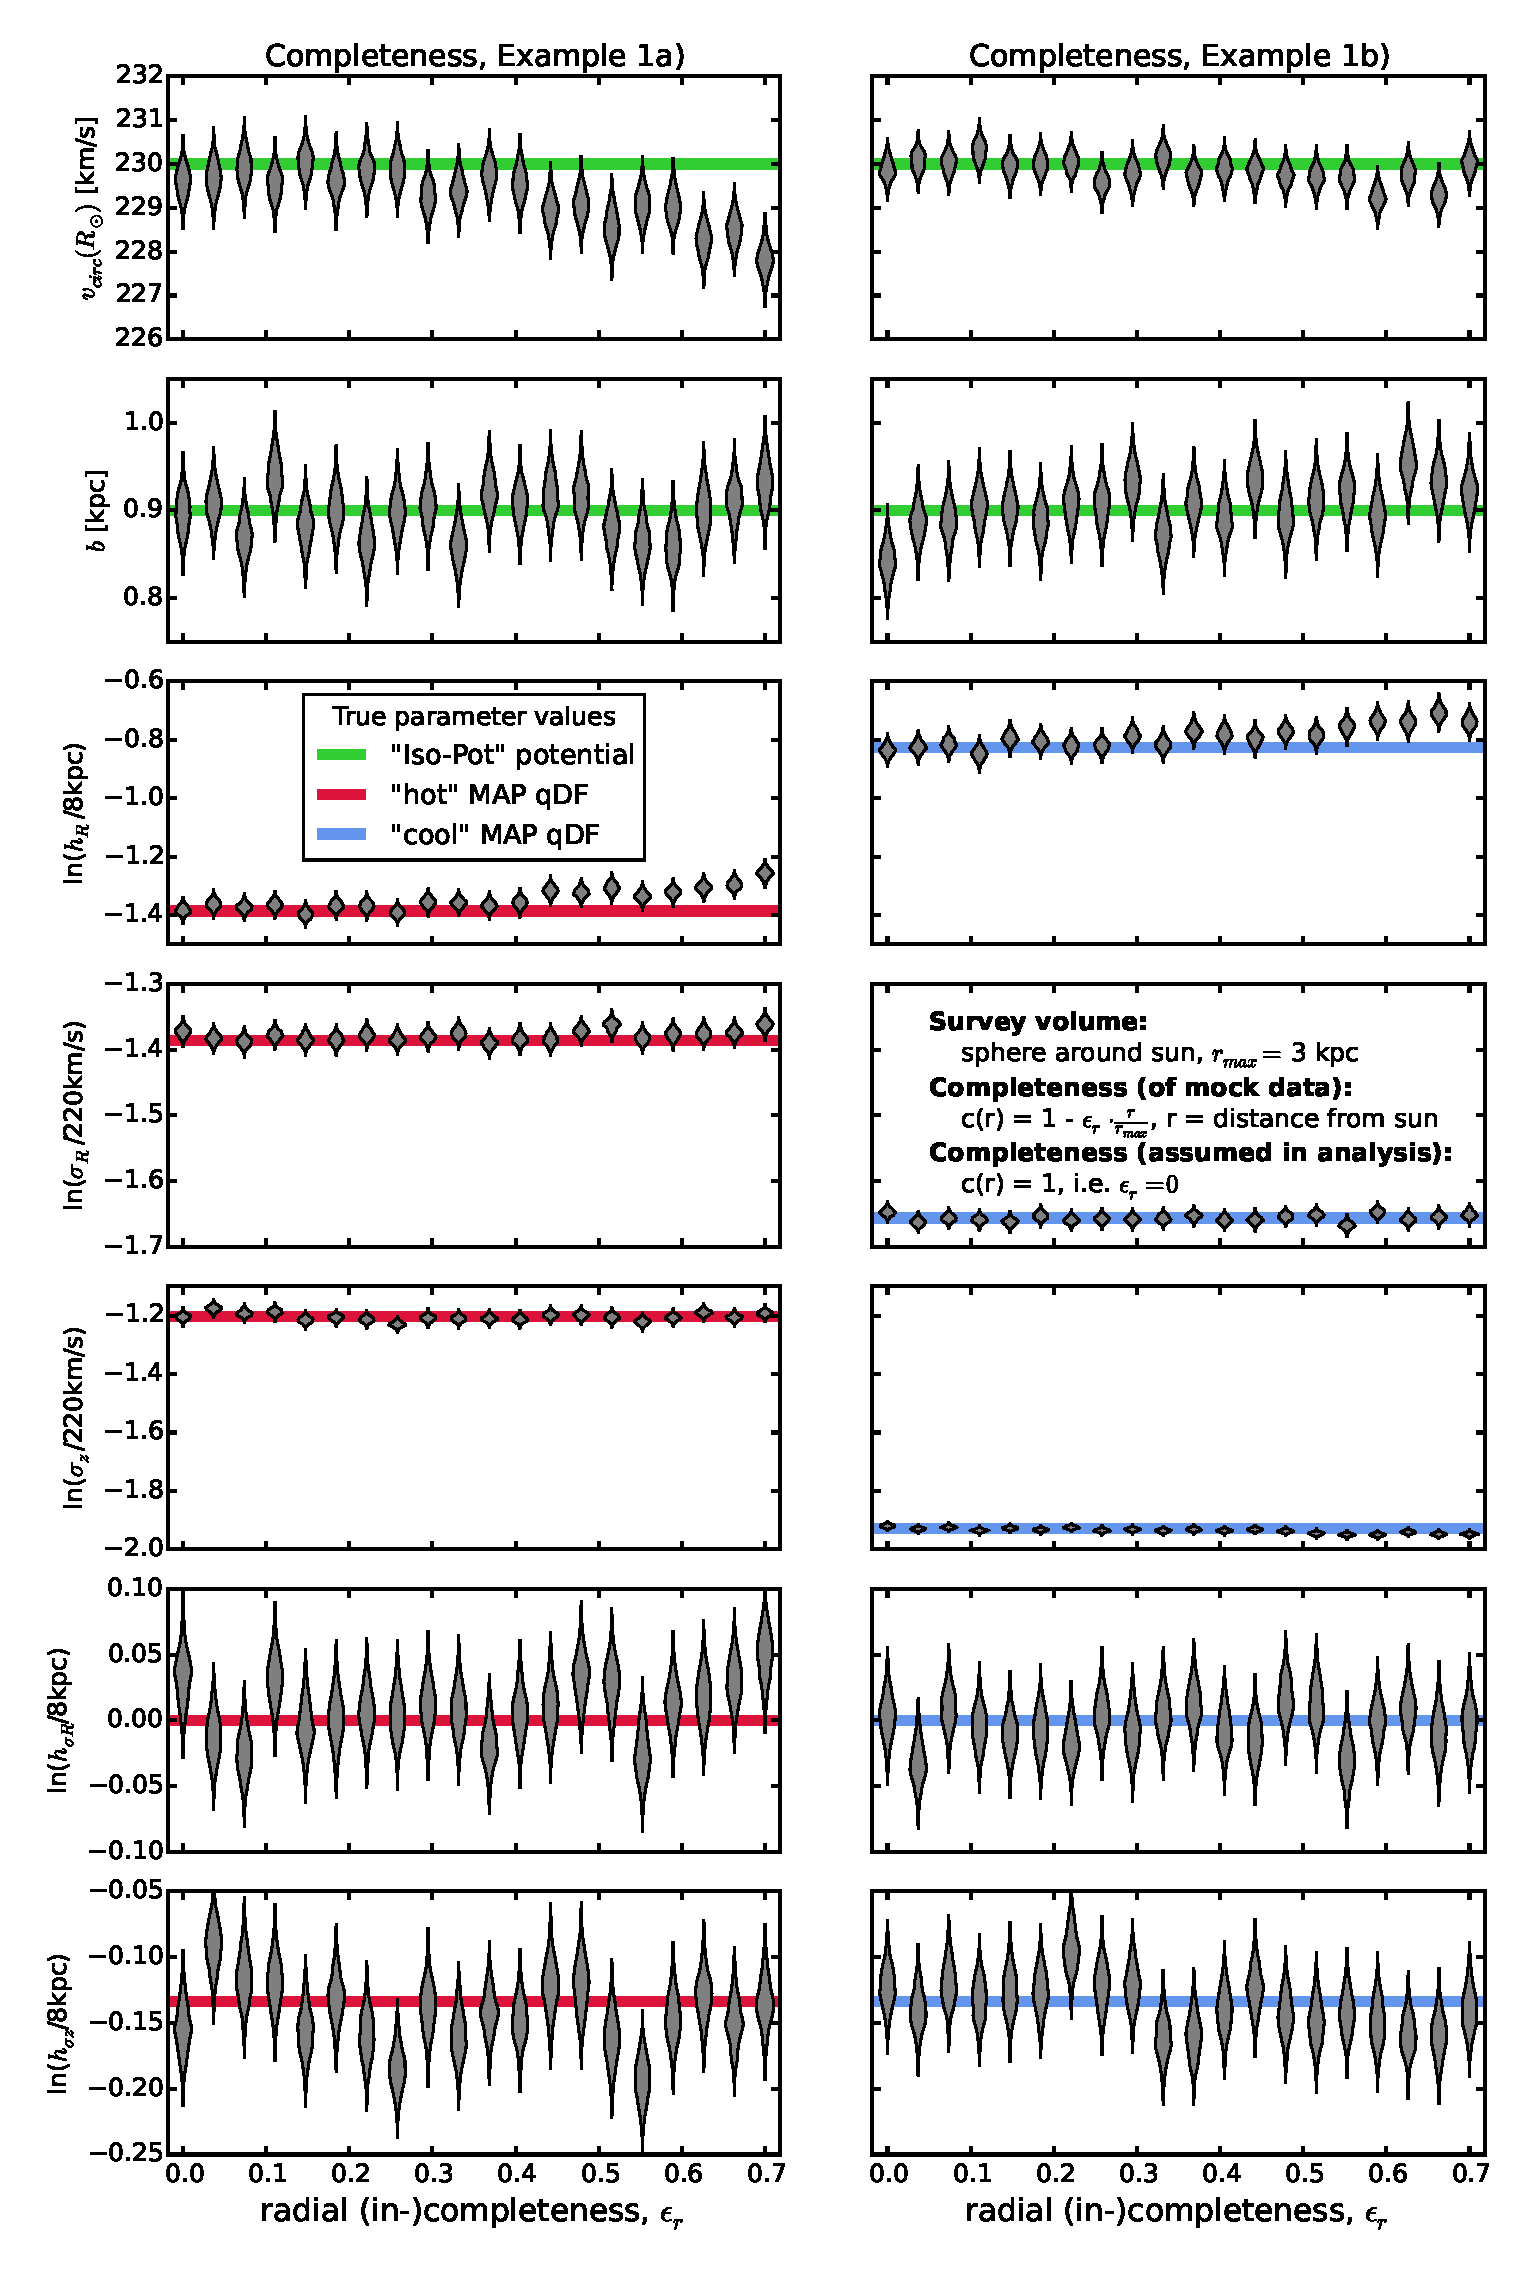
\includegraphics[width=0.8\textwidth]{figs/isoSphFlexIncompR_violins.eps}
\caption{(Caption on next page.)}
\end{figure*}


\addtocounter{figure}{-1}
\begin{figure*} [t!]
\caption{Influence of wrong assumptions about the radial incompleteness of the data on the parameter recovery with \RM. Each mock data set was created having different incompleteness parameters $\epsilon_r$ (shown on the $x$-axis and illustrated in Figure \ref{fig:isoSphFlexIncompR_mockdata}) and the model parameters are given as Test \ref{test:isoSphFlexIncomp}, Example 1, in Table \ref{tbl:tests}. The analysis however didn't know about the incompleteness and assumed that all data sets had constant completeness within the survey volume ($\epsilon_r = 0$). The marginalized likelihoods from the fits are shown as violins. The green lines mark the true potential parameters (\texttt{Iso-Pot}) and the red and blue lines the true qDF parameters (\texttt{hot} \MAP in red and \texttt{cool} \MAP in blue), which we tried to recover. The \RM method seems to be very robust against small to intermediate deviations between the true and the assumed data incompleteness. [TO DO: rename $h_{\sigma R}$ to $h_{\sigma,R}$, $\sigma_R$ to $\sigma_{R,0}$ and analogous for $z$] [TO DO: Potential and/or population names in typewriter font]} 
\label{fig:isoSphFlexIncompR_violins}
\end{figure*}

